% ****** Start of file apssamp.tex ******
%
%   This file is part of the APS files in the REVTeX 4.1 distribution.
%   Version 4.1r of REVTeX, August 2010
%
%   Copyright (c) 2009, 2010 The American Physical Society.
%
%   See the REVTeX 4 README file for restrictions and more information.
%
% TeX'ing this file requires that you have AMS-LaTeX 2.0 installed
% as well as the rest of the prerequisites for REVTeX 4.1
%
% See the REVTeX 4 README file
% It also requires running BibTeX. The commands are as follows:
%
%  1)  latex apssamp.tex
%  2)  bibtex apssamp
%  3)  latex apssamp.tex
%  4)  latex apssamp.tex
%
\documentclass[%
%superscriptaddress,
%groupedaddress,
%unsortedaddress,
%runinaddress,
%frontmatterverbose, 
%preprint,
%showpacs,preprintnumbers,
%nofootinbib,
%nobibnotes,
%bibnotes,
 amsmath,amssymb,
 aps,
 twocolumn,
 prl,
 reprint,
%pra,
%prb,
%rmp,
%prstab,
%prstper,
floatfix,
]{revtex4-1}

\usepackage{graphicx}% Include figure files
\usepackage{dcolumn}% Align table columns on decimal point
\usepackage{bm}% bold math
\usepackage{lineno}
\usepackage{color}
\usepackage{acronym}
\usepackage{multirow}
\usepackage{tabularx}
%\addbibresource{references.bib}
\linenumbers % Commence numbering lines
%\usepackage{hyperref}% add hypertext capabilities
%\usepackage[mathlines]{lineno}% Enable numbering of text and display math
%\linenumbers\relax % Commence numbering lines

%\usepackage[showframe,%Uncomment any one of the following lines to test 
%%scale=0.7, marginratio={1:1, 2:3}, ignoreall,% default settings
%%text={7in,10in},centering,
%%margin=1.5in,
%%total={6.5in,8.75in}, top=1.2in, left=0.9in, includefoot,
%%height=10in,a5paper,hmargin={3cm,0.8in},
%]{geometry}

%% ----- some handy shortcuts
\newcommand{\dcc}{LIGO-PXXXXXXXX}
\newcommand{\optsnr}{\rho_{\mathrm{opt}}}
\newcommand{\fmin}{f_{\mathrm{min}}}

%% ----- comment commands for each of us
\newcommand{\chris}[1]{\textbf{\textcolor{green}{CHRIS: #1}}}
\newcommand{\michael}[1]{\textbf{\textcolor{red}{MICHAEL: #1}}}
\newcommand{\hunter}[1]{\textbf{\textcolor{blue}{HUNTER: #1}}}
\newcommand{\fergus}[1]{\textbf{\textcolor{cyan}{FERGUS: #1}}}

%% ----- result macros - where we store all key results
\newcommand{\cnnsnreight}{97.88}

%% ----- input git-version tag
\input{tag.tex}

\begin{document}

\preprint{APS/123-QED}

%
% Be clear and specific. Do not claim too much or too little.
%
\title{Matching Matched Filtering with Deep Networks in Gravitational wave Astronomy}

\author{Hunter Gabbard}
 \email{Corresponding author: h.gabbard.1@research.gla.ac.uk}
\author{Fergus Hayes}
\author{Chris Messenger}
\author{Michael Williams}
\affiliation{
 SUPA, School of Physics and Astronomy, \\
 University of Glasgow, \\
 Glasgow G12 8QQ, United Kingdom \\
}

%\date{\today}% It is always \today, today,
             %  but any date may be explicitly specified

\date{\commitDATE\\\mbox{\small \commitID}\\\mbox{\dcc}}

%
% Explain what the result is and why it’s important, plus possibly a sentence
% or two of introduction, motivation, methods, caveats.
%
\begin{abstract} 
%
We report on the construction of a deep convoloutional neural network that can
reproduce the sensitivity of a matched-filter search for binary black hole
gravitational wave signals. We report a new method for classifying
gravitational-wave (GW) signals from binary black hole (BBH) mergers using a
deep convolutional neural network. Using only the raw time series as an input,
we are able to distinguish GW signals injected in Gaussian noise amongst
instances of purely Gaussian noise time series with (\textbf{need figure of
merit here}) percent accuracy.  We compare our results with the standard method
of matched filtering used in Advanced LIGO and find the methods to be
comparable.~\chris{I will edit the abstract when we have final results}~\fergus{We need to mention the superior analysing speed in the abstract}
\begin{description} \item[PACS numbers] May be entered using the
\verb+\pacs{#1}+ command.  
\end{description} 
%
\end{abstract}

\pacs{Valid PACS appear here}% PACS, the Physics and Astronomy
                             % Classification Scheme.
%\keywords{Suggested keywords}%Use showkeys class option if keyword
                              %display desired


\maketitle

\acrodef{GW}[GW]{gravitational-wave}
\acrodef{BBH}[BBH]{binary black hole}
\acrodef{SNR}[SNR]{signal-to-noise ratio}
\acrodef{GPU}[GPU]{graphics processing unit}
\acrodef{PSD}[PSD]{power spectral density}
\acrodef{BNS}[BNS]{binary neutron star}
\acrodef{FFT}[FFT]{fast Fourier transform}
\acrodef{CNN}[CNN]{convolutional neural network}
\acrodef{ROC}[ROC]{receiver operator characteristic}

%\tableofcontents

%
% Explain what the result is and why it’s important, particularly arguing how
% the paper will move physics forward. Like the abstract, but shorter and with
% a focus on WHY not HOW.
%

%
% Give sufficient background so the general reader can understand what you did
% and why you did it.
%
\textit{Introduction} --- 
%
% intro to gravitational waves
%
The field of gravitational wave astronomy has seen an explosion of compact
binary coalescence detections over the past several years. The first of these
were binary black hole detections~\cite{PhysRevLett.116.061102,
PhysRevLett.116.241103, PhysRevLett.118.221101} and more recently the advanced
detector network made the first detection of a binary neutron star
system~\cite{PhysRevLett.119.161101} seen in conjuction with a gamma-ray
burst~\cite{2017arXiv171005834L,2017arXiv171005446G,2017arXiv171005449S} and
multiple post-merger electromagnetic signatures~\cite{2017arXiv171005833L}.
These detections were made possible by the Advanced Laser Interferometer
Gravitational wave Observatory (aLIGO) detectors, as well as the recent joint
detection of GW170814 with Advanced Virgo \cite{PhysRevLett.119.141101}. Over
the coming years many more such observations, including \ac{BBH}, binary
neutron stars, as well as other more exotic sources such as intermediate black
holes (IMBH), and neutron star black hole (NSBH) mergers, are likely to be
observed on a more frequent basis. As such, the need for more efficient search
methods will be more pertinent as the detectors increase in sensitivity.

%
% describe the existing algorithms
%
The algorithms used to make these detections \cite{0264-9381-33-21-215004, 0004-637X-748-2-136} are computationally expensive to run.
Part of the reason being that the methods used by these \textit{search
pipelines} are complex, sophisticated processes run over a large parameter
space using advanced signal processing techniques. Distinguishing noise from
signal in this search pipeline, and others like it, is done using a technique
called template based matched filtering. 

%
% introduce matched filtering
%
Matched template filtering uses a \textit{bank} of template waveforms that span
the astrophysical parameter space \cite{PhysRevD.44.3819, PhysRevD.49.1707,
PhysRevD.53.6749, PhysRevD.60.022002, 0264-9381-23-18-002, PhysRevD.80.104014, Blanchet2014, PhysRevD.89.061502}. A template bank will span a large astrophysical parameter space since we do not
know \textit{a priori} what the true parameters of the gravitational waves will
be. The waveforms of the signals are well modeled by post-Newtonian
theory~\cite{PhysRevD.84.049901,PhysRevD.80.084043,Blanchet2014,PhysRevD.93.084054},
and analysis pipelines use matched filtering to search for those signals buried
in the detector noise. More on how we implement this technique and further
comparisons with our model will be described later in this letter.

%
% introduce deep learning
%
Deep learning is a subset of machine learning which has gained in popularity in
recent years~\cite{NIPS2012_4824, 1406.2661, 1409.1556, 1412.7062, 1311.2901,
1409.4842} with the rapid development of \ac{GPU} technology. Some successful
implementations of deep learning have been used in the colorization of black
and white images \cite{1603.08511}, automatic image caption generation
\cite{1412.2306}, object classification and detection in photographs
\cite{NIPS2012_4824}, machine learning for medical diagnosis \cite{KONONENKO200189}, and microarray gene expression classification \cite{Pirooznia2008}. There has also been some recent success in the field of gravitational wave astronomy in the form of glitch classification \cite{0264-9381-34-6-064003,1706.07446} and signal identification \cite{1701.00008}. One
advantage of deep learning is its ability to perform analyses very rapidly
since the method's computationally intensive stage is pre-computed during the
training step prior to the analysis of actual data. This results in low-latency
searches that are several orders of magnitude faster~\cite{726791} than other
comparable classification methods. 

%
% more detail on deep learning
%
A deep learning algorithm is composed of stacked arrays of processing units, called
neurons, which can be anywhere from one to several layers deep. A neuron acts
as a filter, whereby it is passed a vector of inputs, performs a transformation
on them and then outputs a single scalar value. Deep learning algorithms
typically consist of an input layer, followed by one to several hidden layers
and then one to multiple fully-connected neurons. This value
can then either be used to solve classfication, or regression-like problems~\hunter{@fergus, not sure what you're asking here? Insert your statement as new sentence?}~\fergus{Regression is the technique applied for both classification and parameter estimation}. In
the case of classification, each output neuron corresponds to the probability
that a particular input sample is of a certain class.

%
% what are we going to do
%
In this letter we investigate the simplest case of establishing whether a
signal is present in the data or if the data contains only detector noise. We
propose a deep learning procedure requiring only the raw data time
series as input with minimum signal pre-processing. We show how this approach
can be pre-trained using simulated data-sets and applied in low-latency 
to acheive the same sensitivity as established matched filtering techniques. 

%
% the structure of the paper
% 
In the following sections we will discuss our choice of network architecture
and tuning of it's hyperparameters, compare the results of our network with the
widely used matched-filtering gravitational-wave signal classification
technique, and comment on future improvements and applications of this work.      

%
% Try to be clear, e.g. use heuristic explanations. But making a strong case
% for the result takes precedence. You can submit Supplementary Material or,
% better, an accompanying longer paper.
%
\textit{Simulation details} --- 
%
% describe the simulations
%
In order to make a clean comparison between a deep learning approach and
matched-filtering, we distinguish between only 2 cases, \ac{BBH} merger signals
in additive Gaussian noise (signal+noise) and Gaussian noise alone
(noise-only). We choose to focus on \ac{BBH} signals only rather than including
\ac{BNS} systems for the reason that \ac{BBH} systems are higher mass systems
and have shorter duration signals once the inspiralling systems have entered
the Advanced LIGO frequency band. They typically then merge on the timescale of
$\mathcal{O}(1)$ sec allowing us to use a relatively small datasets for this
study. The input datasets consist of simulated gravitational wave timeseries
data that has been whitened in the frequency domain. This process rescales the
noise contribution at each frequency to have equal power resulting in "white"
noise. The signal (if present) has it's constituent frequency components
reweighted according to the \ac{PSD} used.    

%
% describe the noise (Gaussian)
%
Our noise is generated from a \ac{PSD} equivelent to the projected Advanced
LIGO design sensitivity. The \ac{PSD} is used to draw random complex Gaussian
amplitudes to construct frequency series to which we apply an inverse \ac{FFT}
to obtain time domain realisations representing LIGO detector noise.

%
% describe the signal generation 
%
Signals are simulated using a library of gravitational wave data analysis
routines called \texttt{LALSuite}. We use the IMRPhenomD type
waveform~\cite{PhysRevD.93.044006, PhysRevD.93.044007} which models the
inspiral, merger and ringdown components of \ac{BBH} gravitational wave
signals. We simulate systems with component black hole masses in the range from
5\(M_\odot\) to 100\(M_\odot\), $m_{1} > m_{2}$, and all with zero spin. The
specific distribution of masses within these ranges is discussed later on. Each
injection is given a random right ascension and declination assuming an
isotropic prior on the sky, the polarization angle and phase are drawen from a
uniform prior on the range $[0,\pi]$, and the inclination angle is drawn such
that the cosine of inclination is uniform on the range $[-1,1]$. The waveforms
are then randomly placed within the time series, see figure \ref{fig:waveform},
such that the peak of each waveform is then randomly placed within the final $ 20\% $ of the time series. The waveform amplitude is scaled to achieve a predefined optimnal
\ac{SNR} defined as
%
% the optimal SNR
%
\begin{equation} \label{eq:snr} \rho_{\mathrm{opt}}^{2} = 4
\int_{f_{\mathrm{min}}}^{\infty} \frac{\lvert
\tilde{h(f)}\rvert^{2}}{S_{\mathrm{n}}(f)} \mathrm{d}f, \end{equation}
%
where $\tilde{h(f)}$ is the frequency domain representation of the
gravitational wave strain,m $S_{\mathrm{n}}(f)$ is the detector noise \ac{PSD},
and $f_{\mathrm{min}}$ is the frequency at which we start to accumulate
\ac{SNR}. The simulated time series were chosen to be 1~sec in duration sampled
at 8192 Hz and therefore in our case we consider $f_{\mathrm{min}}$ as the
frequency of the gravitational wave signal at the start of the sample
timeseries. An example timeseries can be seen in Figure~\ref{fig:waveform}. 

%
% How we split training, validation, and testing
%
Supervised deep learning approaches to classification problems require
datasets to be sub-divided into training, validation, and testing sets.
Training sets are the data samples that the network learns from, the validation
set allows the developer to verify that the network is learning correctly, and
the test set is used to quantify the performance of the trained network.
Of the datasest generated we use $60\%$ of these samples for training,
$20\%$ for validation, and $20\%$ for testing.

%
% How many sampes did we make
%
Our training datasets contain 50,000 independent timeseries with 50\% containing
signal+noise and 50\% noise-only. For each simulated gravitational wave signal
(drawn from the signal parameter space) we generate 25 independent noise
realisations from which 25 signal+noise samples are produced. This procedure is
standard within machine learning classification and allows the network to learn
how to identify individual signals under different noise scenarios. Each
noise-only sample consists of an independent noise realisation and in total we
use 1000 unique waveforms in the $m_{1},m_{2}$ mass space. Each data sample
timeseries is then represented in the form of a $1 \times 8192$ pixel image
with the grayscale intensity of each pixel proportional to the gravitational
wave amplitude.

%
% explain the distinction on how the masses are distributed 
%
We will only use the training set to teach the deep neural network about the
signals that we wish to classify. For this reason we have chosen to distribute
the masses of the training set according to the density of templates one would
use in a matched filtering approach. It is logical to place waveforms closer in
regions where the waveforms change rapidly and hence we distribute the masses
according to the total mass $M\sim M^{10/3}$ and the symmetric mass ratio
$\eta\sim \eta^{-3}$ where $M=m_{1}+m_{2}$ and $\eta=m_{1}m_{2}/M^{2}$. The
validation, and crucially the testing set must be drawn from distributions that
one would expect to see in nature and we therefore draw those masses from
astrophysically motivated distributions where we assume $m_{1,2}\sim
\log{m_{1,2}}$.   


\begin{figure} 
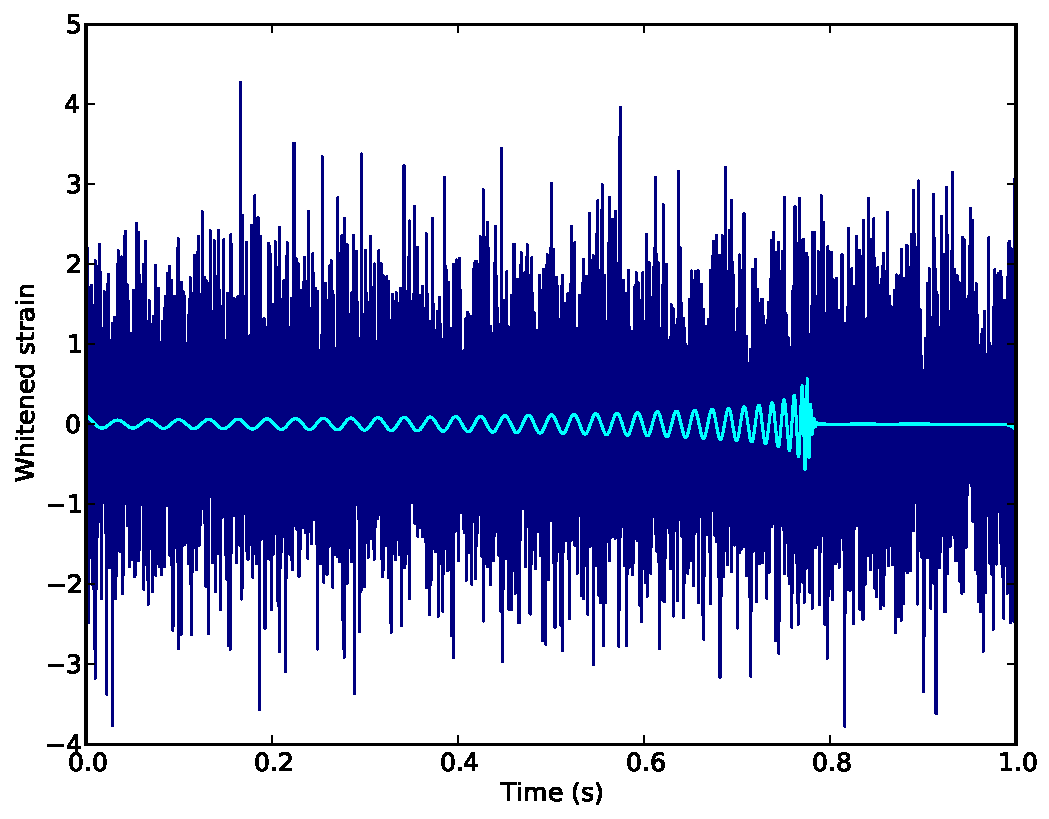
\includegraphics[width=\columnwidth]{figures/waveform.pdf}
\caption{\label{fig:waveform} A whitened noise-free time series of a \ac{BBH}
signal (cyan) with component masses $m_{1}=41.86\mathrm{M}_{\odot}$ and $m_{2}=6.65\mathrm{M}_{\odot}$
with optimal \ac{SNR} 8. The dark blue timeseries shows the
same gravitational wave signal with additive whitened Gaussian noise of unit
variance. This latter timeseries is representative of the datasets we use to
train, validate, and test our deep neural network.} 
\end{figure}

%
% define the CNN structure 
% 
\textit{The Deep Network approach} --- 
%
% introduce convolutional neural networks
%
In our model, we use a variant of a deep learning algorithm called a
\ac{CNN}~\cite{726791}. The layers of such a network are composed of five
primary variants: input, convolutional, activation, pooling, and
hidden. The input layer holds the raw pixel values of the sample
image which in our case is a 1-dimensional timeseries vector.  Each neuron in
the convolutional layer computes the convolution between an as yet undefined
kernel or vector of pixel values and the outputs from the layer above it. A neuron has
its own characteristic set of weights and bias vectors (being the same dimension as that of the input vector). The input vector is multiplied element-wise with the neuron's weight vector and then summed together with the neuron's bias vector. Neuron weight vectors are updated through an optimisation algorithm called back-propogation \cite{LeCun1998}. 
Activation layers apply an element-wise non-linear activation function rescaling
their inputs onto the range $[-1,1]$ and leaving the size of the previous
layer's output unchanged. The activation function can be shifted to better fit network predictions by adjusting the bias vector. 
Pooling layers perform a downsampling operation along
the spatial dimensions of their input essentially acting as a data reduction
process speeding up the training of the network for minimal loss of
information. Finally we have a hidden layer which connects to a final output layer that
computes the class scores using an error function, cross-entropy, defined as
%
% define the loss function
%
\begin{equation} \label{eq:loss}
f_{\theta^{'}}(\theta) = -\sum_{i} \theta_{i}^{'} \mathrm{log}(\theta_{i}),
\end{equation}
%
where $\theta_{i}$ is the predicted probability distribution of class $i$ and
$\theta_{i}^{'}$ is the true probability for that class
\cite{tensorflow2015-whitepaper}. The error function computes the inefficiency of
the network predictions with respect to the true value. 

%
% describe the network choices that we have
%
In order to optimise our network, multiple sets of hyper-parameters are
tuned. We define hyper-parameters as those parameters that we are free to
choose. Such parameters include the choice of the number and type of network
layers, the number and size of neurons within each layer, the max-pooling
parameters, the type of activation functions, preprocessing of input data,
 learning rate, and the application (or otherwise) of specific deep learning techniques. We begin
the entire process with the simplest network that provides a discernable level
of effective classification. In most cases this consists of an input,
convolutional, hidden, and logistic output layer.

%
% go into more detail about what we tried in network design
%
Within our optimisation process we experimented with rescaling the input data
which we found to have minimal effect on the network performance. The reason
for this is that our input data is whitened and our signals are buried beneath
the noise. Therefore our data is essentially prescaled on a range
$\pm\mathcal{O}(1)$ due to the natural variation of Gaussian noise. We also
attempted applying transfer learning \cite{5288526}
where we used networks pre-trained on high \ac{SNR} datasets as starting points
for application to successively lower \ac{SNR} datasets. We found that there
were no performance benefits using this approach.  Network depth was adjusted
between 2 and 10 convolutional layers. The
inclusion of dropout was used within the fully-connected layers as a form of
regularization.

%
% describe how the training itself works to optimise the weights and biases
%
For updating our weights and bias parameters (in
order to minimize our loss function, $f(\theta)$, \eqref{eq:loss}) we settled
on the Nesterov momentum optimization function. The optimisation function (back-propogation) works by
computing the gradient of the loss function, then attempting to minimise 
that loss function. The errors are then propogated back through the network while at the same time 
updating the weight and bias terms accordingly.  Back propogation is done over multiple iterations called \textit{epochs}. 

%\begin{equation} \label{eq:nesterov1}
%v_{i+1} = \mu v_{i} - \epsilon \nabla f(\theta_{i} + \mu v_{i}),
%\end{equation}

%\begin{equation} \label{eq:nesterov2}
%\theta_{i+1} = \theta_{i} + v_{i+1},
%\end{equation} \\

Nesterov momentum was the ideal choice because of its prescient ability to
approximate the next position of the weights and bias parameters which
therefore gives a rough approximation of their future values
\cite{Sutskever:2013:IIM:3042817.3043064}. Further detailed description of the
neural network architecture used can be found in
Table~\ref{table:network}. 

The ranking statistic that we extract from the CNN analysis is taken from the final output layer,
composed of 2 neurons, where each neuron will output a probability value bewteen zero and 1. One neuron gives the probability that a signal is noise and the second gives the probability that the signal is astrophysical. This output is then used to classify our signals.

\begin{figure} 
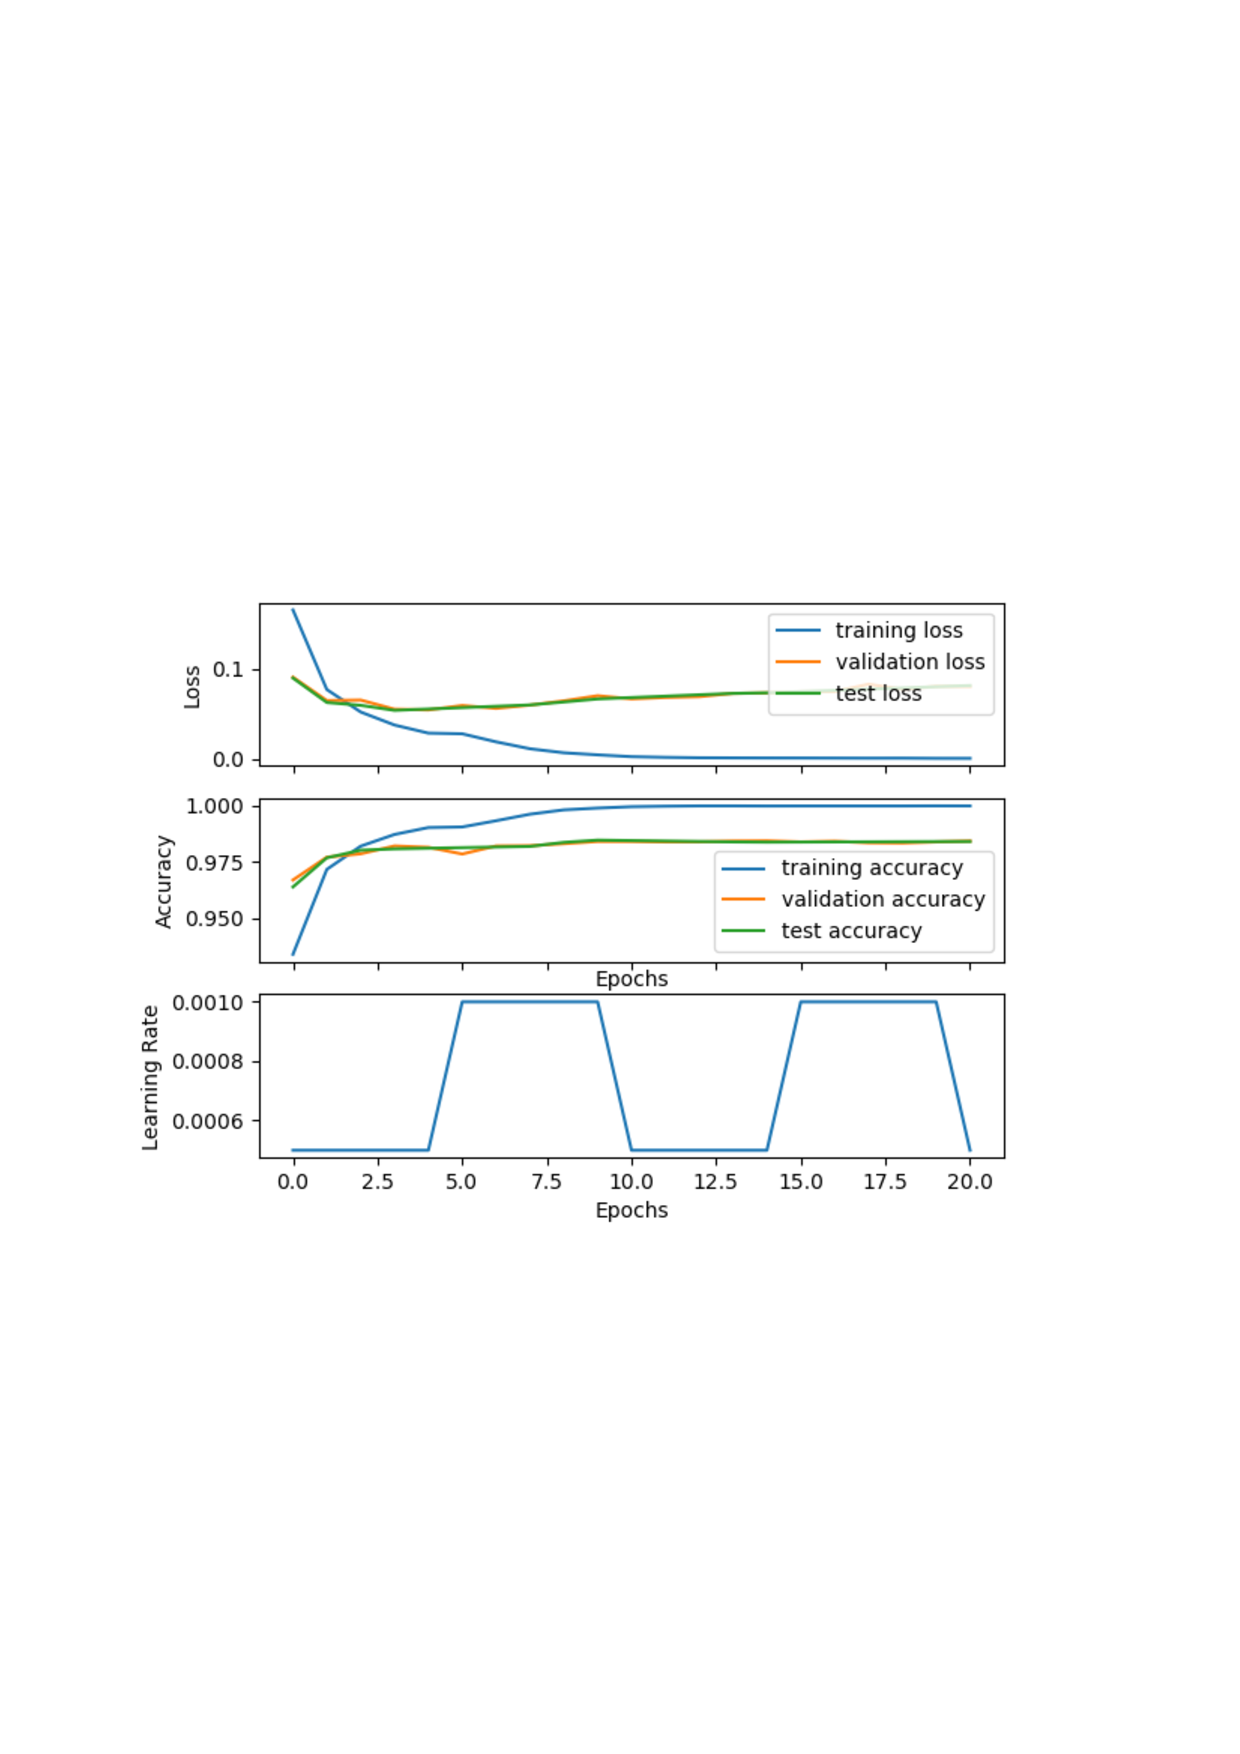
\includegraphics[width=\columnwidth]{figures/loss.pdf}
\caption{\label{fig:loss_curve} \hunter{Not sure if we stil need this figure? I'd still like to keep it though} The
loss, accuracy and learning rate~\chris{in the main text none of these
quantities seem to be defined. This is a problem!} plots (shown above)
illustrate how the network's performance is defined as a function of the number
of training epochs. The goal is
to minimize the loss function, which will in turn maximize the accuracy of the
classifier. The first initial epochs see an exponential decrease in the loss
function and then a slowly falling monotonic curve to follow. This indicates
that the longer our network is trained, a limit with respect to the accuracy is
approached. In our case, we cyclically adjust the learning rate to oscilate
between $5 \times 10^{-4}$ and $1 \times 10^{-3}$ at a constant frequency.
Studies have shown that this policy of learning rate adjustement.~\chris{Also
define exactly what run this was run on, what accuracy and loss were achieved
and make sure that you show the typical number of epochs used in the analysis.
Maybe use log-scale on the y-axis of the loss plot.}} 
\end{figure}

\begin{table}[]
\begin{tabular}{lcccccccccc}
\hline
\hline
Parameter & \multicolumn{10}{c}{Layer}\\
\cline{2-11}
(Option) & 1 & 2 & 3 & 4 & 5 & 6 & 7 & 8 & 9 & 10 \\
\hline
Type & C & C & C & C & C & C & C & C & H & H \\
No. Neurons  & 8  & 16  & 16 & 32 & 64 & 64 & 128 & 128 & 64  & 2  \\
Filter Size  & 32 & 16  & 16 & 16 & 8  & 8  & 4   & 4   & n/a & n/a \\
MaxPool Size & yes & no & no & no & yes & no & no & yes & no & no \\
Drop out  & 0 & 0 & 0 & 0 & 0 & 0 & 0 & 0 & 0 & 0.5 \\
Act. Func. & Elu & Elu & Elu & Elu & Elu & Elu & Elu & Elu & Elu & SMax \\
\hline
\end{tabular}
\caption{The optimal network structure was determined through multiple tests
and tunnings of hyperparameters by means of trial and error. The network
consists of 8 convolutional layers (C), followed by 2 hidden layers (H).
Max-pooling is performed on the first, fifth, and eighth layer~\chris{can you
replace the yes/no entrieds for max-pooling with the pool sizes please?},
whereas dropout is only performed on the two fully-connected layers. Each layer
uses an Elu activation function while the last layer uses a Softmax activation
function in order to normalize the output values to be between zero and one so
as to give a probability value for each class.\label{table:network}}
\end{table}

%
% define the matched filter analysis
%
\textit{Applying matched-filtering} ---
%
% introduce matched filtering
%
In order to establish the power of the deep learning approach we must compare
our results to the standard matched filtering process used in the detection of
compact binary coalescence
signals~\cite{PhysRevD.85.122006,2013PhRvD..87b4033B}. The ranking statistic
used in this case is the matched-filter \ac{SNR} analytically maximised over
arrival time, phase and distance. By first defining the noise weighted inner
product as a function of a time shift $\Delta t$ between the arrival time of
the signal and the template,
%
% define the matched-filter SNR
%
\begin{equation}
(a\mid b)[\Delta t] =
4\int_{f_{\mathrm{min}}}^{\infty}\frac{\tilde{a}(f)\tilde{b}^{*}(f)}{S_{\mathrm{n}}(f)}e^{2\pi i
f\Delta t}\,df,
\end{equation}
%
we can construct the matched-filter \ac{SNR} as 
%
\begin{equation}
\rho^{2}[\Delta t]=\frac{(s\mid h)^{2}[\Delta t] + i(s\mid h)^{2}[\Delta t]}{(h\mid h)}
\end{equation}
%
where $s$ is the data containing noise and a potential signal and $h$ is the
noise-free gravitational wave template. For a given template this quantity is
efficiently computed and $\Delta t$ maximised over using \acp{FFT}.  All that
remains is to further numerically maximise this quantity over a template of
component mass combinations. In this analysis a comprehensive template bank is
generated in the $m_{1},m_{2}$ mass space covering our predefined range of
masses and with a mismatch of $?\%$ using the PyCBC tools~\chris{need a
reference}. The template bank in this case contains $?$ individual templates. 

%
% describe the process of what we apply this to
%
For the practical computation of the matched-filter analysis we take each of
the data samples from the testing dataset and compute the time, phase and
amplitude maximised ranking statistic $\rho$ for each template in the bank. We
then record the value of $\rho$ maximised over each template. With values of
statistics now assigned to each test data sample from both the
matched-filtering and \ac{CNN} approaches, and having knowledge of the
true class associated with that sample, we may now contruct \ac{ROC} curves.  

%
% Describe the main results of the study
%
\textit{Results} --- 
%
% introduce the confusion matrix results
%
A standard method for displaying the accuracy of a classifier is through a
confusion matrix in which the number of samples of each true class identified
as every possible class are listed in a square matrix. A fully diagonal matrix
would imply no incorrectly classified samples and a uniform matrix would imply
no classification power. In Figure~\ref{fig:confusion} we show results for the
\ac{CNN} approach from which we highlight the overall accuracy (the ratio of
incorrectly identified samples to the total number of samples) of
\cnnsnreight\% at $\rho_{\mathrm{opt}}=8$.

%
% a description of the transfer learning approach (do we need this?)
%
\chris{remove this paragraph?} After tunning several hyperparameters and then settling on
an ideal network format (Table \ref{table:network}), we present the results of
our classifier on a noise vs. signal+noise sample set. We trained our network
using a transfer learning approach whereby we initially trained our network on
a sample set of 1,000 noise and 1,000 injection signals (each with 25 different
noise realizations) with an integrated SNR value of 12. We then lowered the
integrated SNR value by 2 and (using the same weights from our previous
network) we trained our classifier again. This approach seemed to only have a
marginal benefit on the overall performance of the classifier~\chris{Do we
actually do this? Does it make the results better OR does it simply speed the
process up? Earlier on in the paper we say that we don't use it. If it doesn't
actually change our results then we shoud remove most of this paragraph.}  

%
% confusion matrix plot
%
\begin{figure}[]
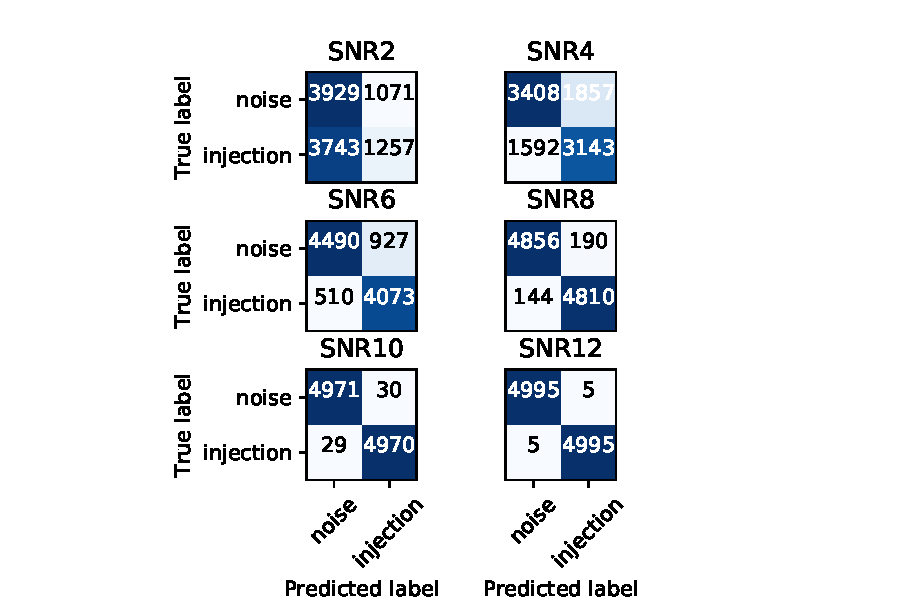
\includegraphics[width=\columnwidth] {figures/confusion_matrix.pdf}
\caption{Confusion matrices for testing datasets containing signals with
optimal SNR $\rho_{\mathrm{opt}}=2,4,6,8,10,12$.  Numbers superimposed within
matrix elements are the number of samples corresponding to samples that were of
true class indicated by the y-axis label but identified as the corresponding
x-axis label. For our 2 class system these are equivelent to the numbers of
true positive, true negative, false negative, or false positive. The accuracy
percentages for all injection SNR values are listed as follows: $50.19\%$ at
$\optsnr=2$, $68.34\%$ at $\optsnr=4$, $88.72\%$ at $\optsnr=6$, $97.88\%$ at
$\optsnr=8$, $99.64\%$ at $\optsnr=10$ and $99.86\%$ at
$\optsnr=12$.\chris{maybe plot 2x3 rather than 3x2 if we have the space. Also
we habve to anser the question of why the SNR=2 case mostly predicts an signal,
why are there not equal numbers in each element as you would
expect?}\label{fig:confusion}}
\end{figure}

%
% describe ROC curves
%
In Figure~\ref{fig:ROC_curves} we compare our \ac{CNN} results to that of
matched filtering. Given the ranking statistic from a particular analysis and
defining a parametric threshold value on that statsistic we are able to plot
the fraction of noise samples incorrectly identified (false alarm or false
positive probability) as signals versus the fraction of signal samples
correctly identified (true alarm or true positive probability). These curves
are defined as \ac{ROC} curves and a ranking statistic is deemed superior to
another if at a given false alarm probability it acheives a higher detection
probability. Our results show that within our uncertainties the \ac{CNN}
approach matches the sensitivity of matched filtering for all test datasets
across the full range of false alarm probabilities explored in this
analysis\footnote{We are limited to a minimal false alarm probability of $\sim
10^{-4}$ due to the limited number of testing samples used.}. We also plot as a
reference, the \ac{ROC} curve corresponding to a matched filter analysis for
which the true masses and arrival time of the signal is known. In this case
there is only a single template and the sensitivity is consequently improved.  

%
% Alternative ROC/efficiency results
%
\chris{I advise removing this paragraph} In Figure~\ref{fig:ROC_curve} we
compare our results to that of matched filtering where we use two alternative
match filtering methods.  The first, using the nominal template bank described
in the \textit{Sample Simulation Methods} section, whereas the second uses the
optimal template for each injection, whereby optimal is defined as the template
used to generate that injection. As seen in figure \ref{fig:ROC_curve} all
three methods have equivalent performance proficiency at $\sim \mathrm{iSNR} >
9$, whereas there is a marginal dip in performance in the nominal matched
filtering method and our deep learning classifier. It should be noted that our
classifier exceeds the performance proficiency of that of the nominal matched
filtering method between iSNR 2 and iSNR 4.\chris{I rewrote this paragrpah
above. I thought that there was too much emphasis on the single template
approach and no descriptiuon of he ROC curve. There is also a statement about
us beating matched filtering as low SNR. This is tentative at the moment and
also, if true, annoyingly at low SNR.  Let's wait and see the final results
before we say things contraversial. Also you were describing the efficiency
curves and not the ROC curve which should come first sine the efficiency is
derived from the ROC.} 

%
% show ROC curves
%
\begin{figure}[]
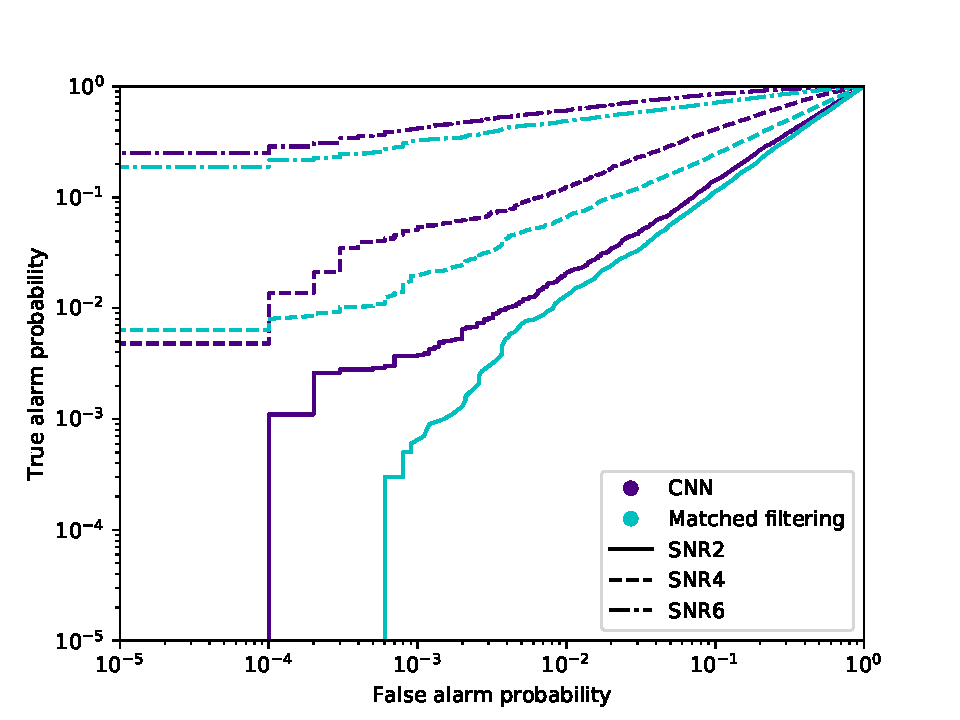
\includegraphics[width=\columnwidth] {figures/ROC_curves.pdf}
\caption{The \ac{ROC} curves for test datasets containing signals with optimal
SNR $\rho_{\mathrm{opt}}=2,4,6,8,10,12$.  In each panel we plot the detection
probability as a function of the false alarm probability estimated from the
output of the \ac{CNN} (blue) and matched-filtering (red) approaches. We also
plot the \ac{ROC} ciurves corresponding to a single template matched-filter
analysis (dashed green).~\chris{OK, first can we make these plots 2x3 rather
than 3x2 so that they are easier to see. Please put the SNR labels inside the
plots rather than on top of them. No need to have dashed curves here so make
the CNN and matched-filter curves solid. Ditch the legend and make the y-axes
log -scale. That should be enough to get on with.\label{fig:ROC_curves}}}
\end{figure}

%
% finally discuss the efficiency plot
%
We can make an additional direct comparison between approaches by fixing a
false alarm probability and plotting the corresponding detection probability
versus the optimal SNR of the signals in each test dataset. We show these
efficiency curves in Figure~\ref{fig:efficiency_curves} at 3 different false alarm
probabilities $10^{-1},10^{-2},10^{-3}$ for both the \ac{CNN} and
matched-filtering approaches. Since these efficiency curves are derived from
the data used to generate the \ac{ROC} curves shown in
Figure~\ref{fig:ROC_curves} it is not surprising that the \ac{CNN} and
matched-filtering approaches produce indistinguishable results (within our
uncertainties) at all choices of false alarm probability.

\chris{Same here, I suggest removing this paragraph} We compare the results of
all three methods at various injection iSNR values in figure
\ref{fig:isnr_curves}. It is not surprising to see that the matched filtering
method using the optimal template consistantly performs better than both the
nominal match filtering method and our deep learning classifier.  However, what
is considerable is the comparison between the nominal matched filtering and the
deep learning classifier detection probability curves. It can clearly be seen
that our classifier exceeds the performance of the nominal matched filtering
method at iSNR 2, 4 and 6. This is a promising result and certainly merits
further investigation.~\chris{I've kind of rewritten this paragraph above for
the same reasons as used for the ROC curves. We just want to stick to the
process of describing what we're plotting and dispassionately pointing out the
key result. No need to again highlight the single-filter result which is only
there for reference.}  

%
% show efficiency curve
%
\begin{figure}[]
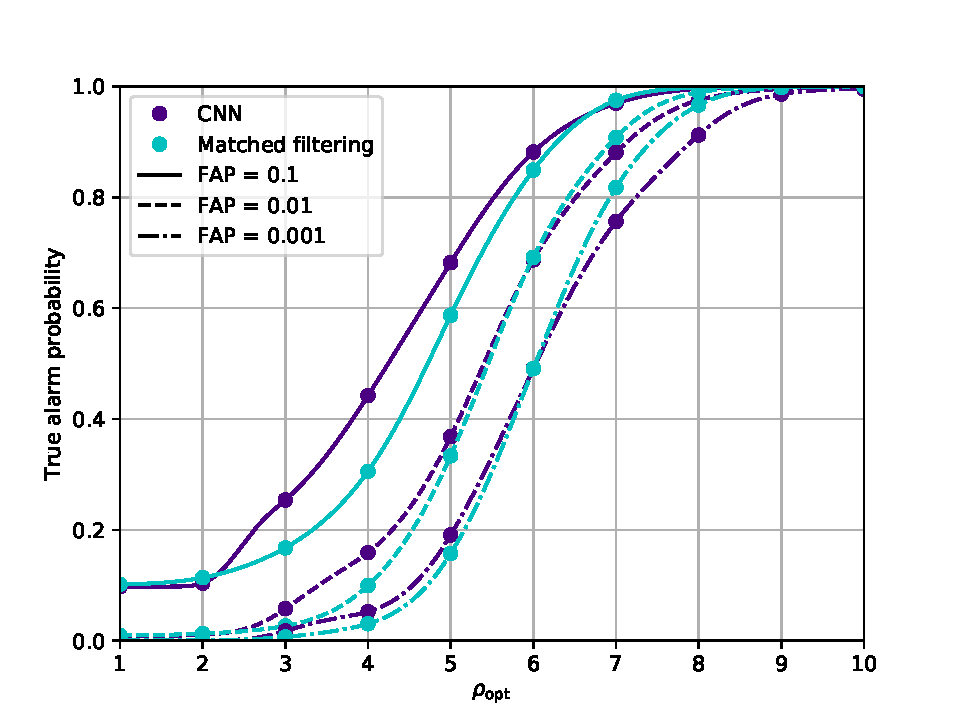
\includegraphics[width=\columnwidth] {figures/efficiency.pdf}
\caption{Efficiency curves comparing the performance of the \ac{CNN} and
matched-filter approaches for a selection of false alarm probabilities. The
detection probability is plotted as a function of the optimal \ac{SNR} for the 
\ac{CNN} (blue) and the matched-filtering (red) analyses. Each collection of
curves is labelled with the corresponding false alarm probability and in each
case for reference we also plot curves for the single template matched-filter
case (green dashed).~\chris{So can we change the x-axis ranges to span exactly 2-12
and the y-axis to span exactly 0-1. Can we label the x-axis as $\optsnr$. Can
we produce 3 sets of results for false alarm probabilities 0.001,0.01,0.1 and
see what the plot looks like with 9 curves (each group of 3 labelled with the
corresponding false alarm probability? Also change legend to say CNN rather
than deep network. Finally change the colours?}\label{fig:efficiency_curve}}
\end{figure}

%
% Summarise what you did, note key equations and specific results. If there is
% a main numerical result, quote it here. Then go back and make sure the
% abstract contains the most important results. Say what’s next
%
\textit{Conclusions} --- 
%
% summary of what we did
%
We have demonstrated that deep learning, when applied to a raw
gravitational-wave timeseries data, is able to reproduce the results of a
matched-filtering analysis in Gaussian noise. We employ a deep convolutional
neural network with carefully chosen hyperparameters and produce an output that
returns a ranking statistic equivelent to the probability that data contains a
signal. Matched filter analyses are often described as the optimal approach for
signal detection in Gaussian noise. By building a neural network that is
capable of reproducing this optimality we answer a fundamental question
regarding the applicability of neural networks for gravitational wave data
analysis. 

%
% Non Gaussian noise
%
In practice, searches for transient signals in gravitational wave data are
strongly affected by non-Gaussian noise artefacts. To account for this,
standard matched filtering approaches are modified to include carefully chosen
changes to the ranking statistic together with the excision of poor quality
data~\chris{we should cite a detchar paper or Toms new-snr paper}. Our analysis
represents a starting point from which a deep network can be trained on
realistic non-Gaussian data with the potential aim of exceeding the sensitivity
of existing matched filter approaches.

%
% Other sources and final statement
%
In this work we have presented results for \ac{BBH} mergers, however, this
method could be applied to other merger types, such as \ac{BNS} and neutron
star-black hole signals. This supervised learning approach can also be extended
to other well modelled gravitational wave targets such as the continuous
emission from rapidly rotating non-axisymmetric neutron stars~\chris{cite the
LIGO O1 or O2 einstein at home paper}. Whereas unsupervised approaches have the
potential to be powerful detection tools in searches for unmodelled burst-like
gravitational-wave signals. 

%
% acknowledge peopkle and funding agencies
%
\emph{Acknowledgements}---We would like to acknowledge valuable input from the
LIGO-Virgo Collaboration specifically the machine-learning working group. The
authors also gratefully acknowledge the Science and Technology Facilities
Council of the United Kingdom.  CM is supported by the Science and Technology
Research Council (grant No.~ST/~L000946/1).
%
%\end{acknowledgments}


% The \nocite command causes all entries in a bibliography to be printed out
% whether or not they are actually referenced in the text. This is appropriate
% for the sample file to show the different styles of references, but authors
% most likely will not want to use it.

\bibliographystyle{apsrev4-1}
\bibliography{references}% Produces the bibliography via BibTeX.


\end{document}
%
% ****** End of file apssamp.tex ******
